\section{A felület elérése}

A kliens oldali program két féle módon is elérhető a felhasználók számára:
\begin{itemize}
  \item Tetszőleges internetböngészővel rendelkező eszközről a helyi hálózaton
  futó szerver segítségével. Ekkor a böngésző címsorába beírva a szerver címét
  egyből a FlockWave kliens felületét kapjuk, ami egy SPA (Single Page
  Application), tehát összesen egy lapból áll, nem alkalmaz navigációt.
  \item Windows, Linux vagy MacOS (OSX) rendszerek alatt Electron segítségével
  becsomagolt állománnyal rendelkező önálló alkalmazásként.
\end{itemize}

A felület megnyitása után szükséges csatlakozni a drónokkal történő közvetlen
kommunikációt végző FlockWave szerver alkalmazást futtató számítógéphez. Ez
lehetséges az elérési cím és port (alapértelmezetten 5000) manuális megadásával,
illetve az SSDP (Simple Service Discovery Protocol) hálózati felderítési
protokoll segítségével.

\section{A felület kezelése}

\subsection{Kezdeti állapot}

Alapállapotban a felület a térképet jeleníti meg, mellette pedig az eltárolt
pozíciók kezelésére alkalmas panelt, valamint az ismert drónok listáját. További
felületi elemek érhetőek el a fülekre kattintva, illetve a bal oldalon található
sávról ( \ref{fig:initial_state}. ábra /\circled{1}) kattintással vagy húzással
a felületre helyezve.

\begin{figure}[H]
  \center
  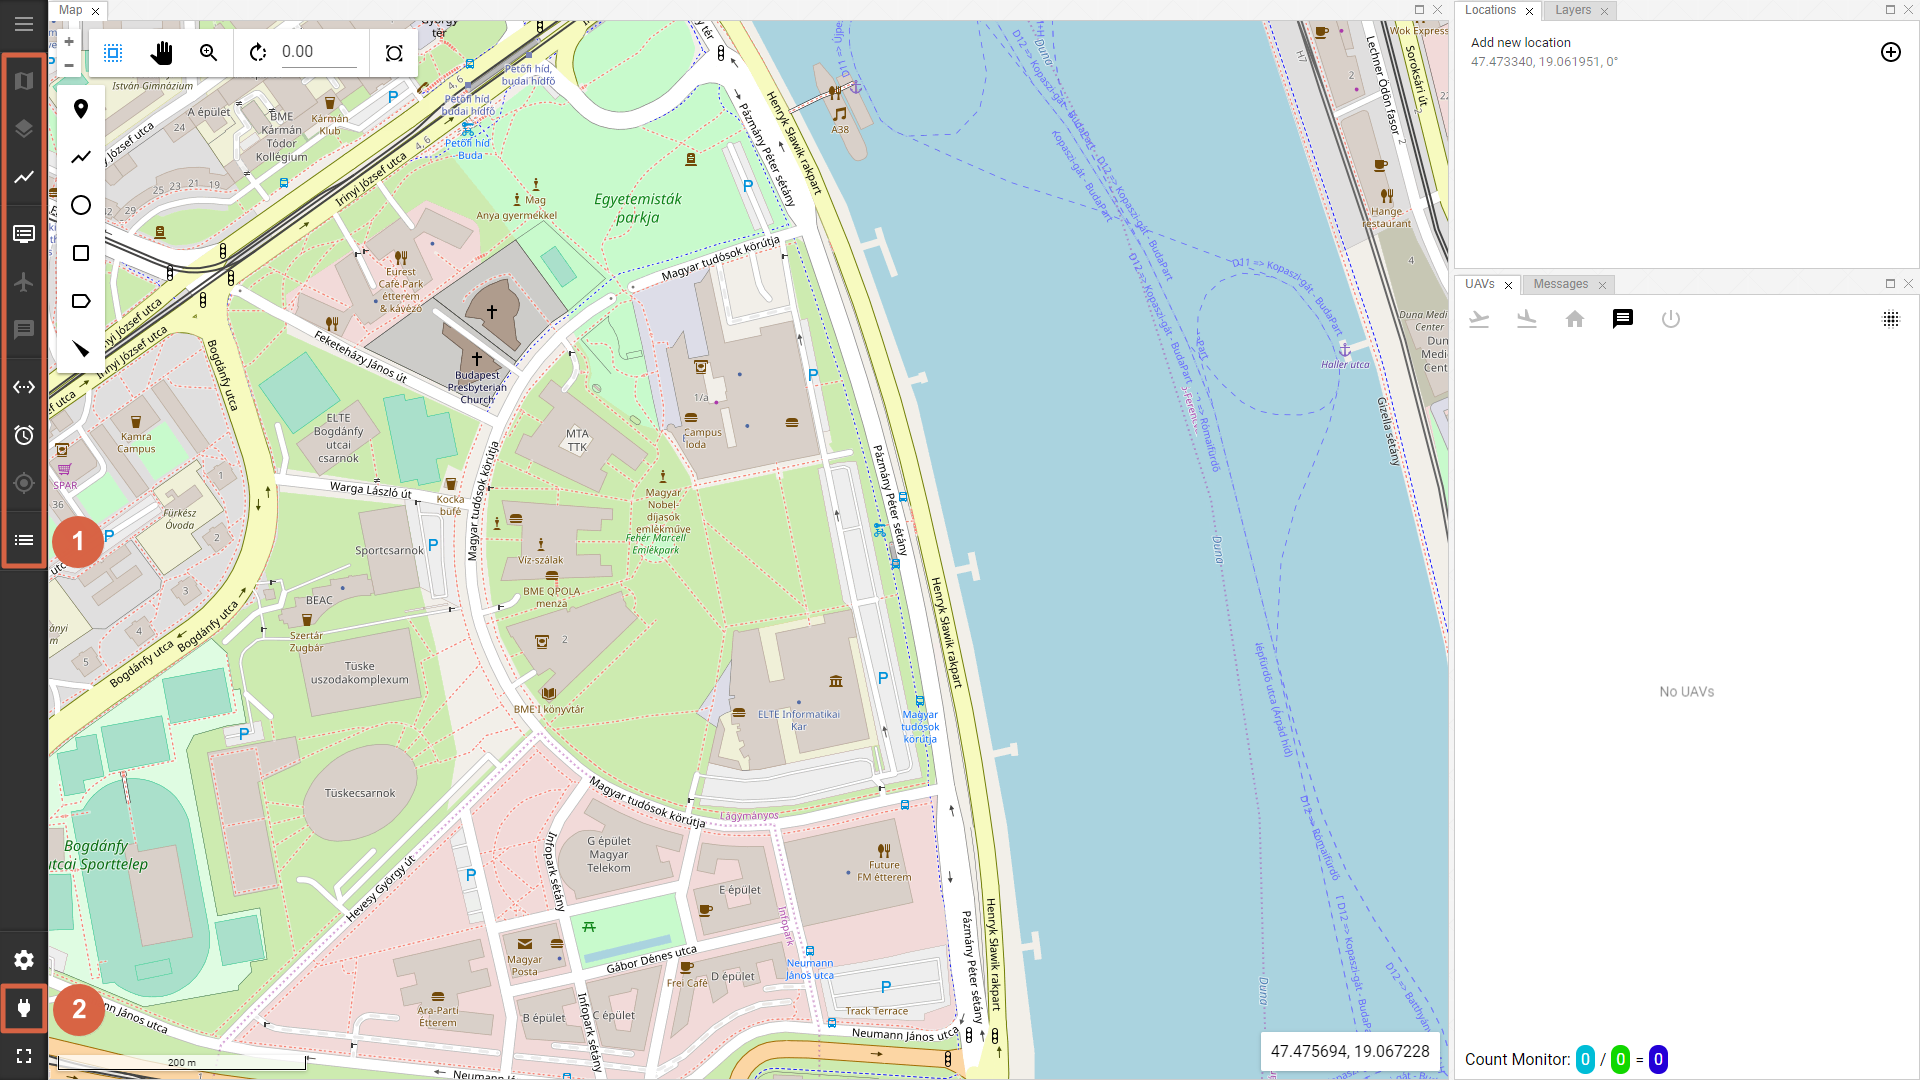
\includegraphics[width=\textwidth]{screenshots/initial_state.png}
  \caption{A kliens program alapállapota}
  \label{fig:initial_state}
\end{figure}


\subsection{Csatlakozás a szerverhez}

A szerverhez való csatlakozásához meg kell adni annak elérési adatait. Ezt a
\ref{fig:initial_state}. ábra /\circled{2} jelölésű gombján történő kattintás
után megjelenő dialógusablakban tehetjük meg.

\begin{figure}[H]
  \center
  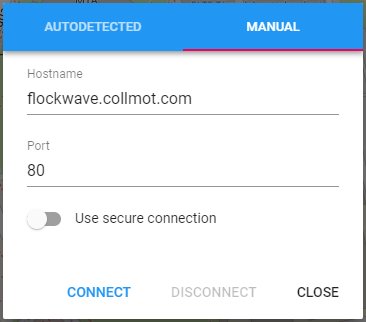
\includegraphics[width=0.5\textwidth]{screenshots/connection_dialog.png}
  \caption{A szerverhez való csatlakozásra szolgáló dialógusablak}
  \label{fig:connection_dialog}
\end{figure}

Sikeres csatlakozás esetén a dialógusablak megnyitására szolgáló gomb mellett
megjelenik egy kis zöld színű teli kör alakú jelölő, az UAVs című panelben és a
térképen pedig láthatóvá válnak a szerverrel aktuálisan kapcsolatban álló
drónok.


\subsection{Hőtérképes megjelenítés}

Hőtérképes megjelenítés segítségével a drónokon elhelyezett műszerek mérései
ábrázolhatóak vizuális módon. Ehhez először egy hőtérkép típusú réteg
létrehozása szükséges a rétegek panelen az "Add new layer", majd pedig azon
belül a "Heatmap" opciót választva.

Ekkor a rendszer lehetőséget biztosít a megfigyelni kívánt csatornákra történő
fel-- és leiratkozásra. Ez az "Edit subscriptions" gomb által megjeleníthető
dialógusablakban tehető meg.

Beállítható továbbá egy küszöbszint, ami alatt az értékeket fehérrel jelzi,
valamint a színskála két széléhez tartozó érték is megadható manuálisan, vagy
pedig bekapcsolható az automatikus skálázás, amely esetén minden beérkező érték
feldolgozásakor frissíti a határokat a rendszer, amennyiben ez szükséges.
Személyre szabhatóak a színskála végpontjainak színárnyalatai, valamint a
színezési függvény is kiválasztható. (Lineáris vagy logaritmikus.)

Ezen felül megadható a mérési pontok közötti minimális távolság, bekapcsolható a
rácspontokhoz történő igazítás, továbbá törölhetőek az eddigi mérési adatok.

A kép (\ref{fig:heatmap}. ábra) például egy logaritmikus színezésű, 5 méteres
sűrűségű rácspontokra igazított hőtérkép látható, amely egy szimulált pontszerű
forrásból származó radioaktív mérés eredményeit ábrázolja.

\begin{figure}[H]
  \center
  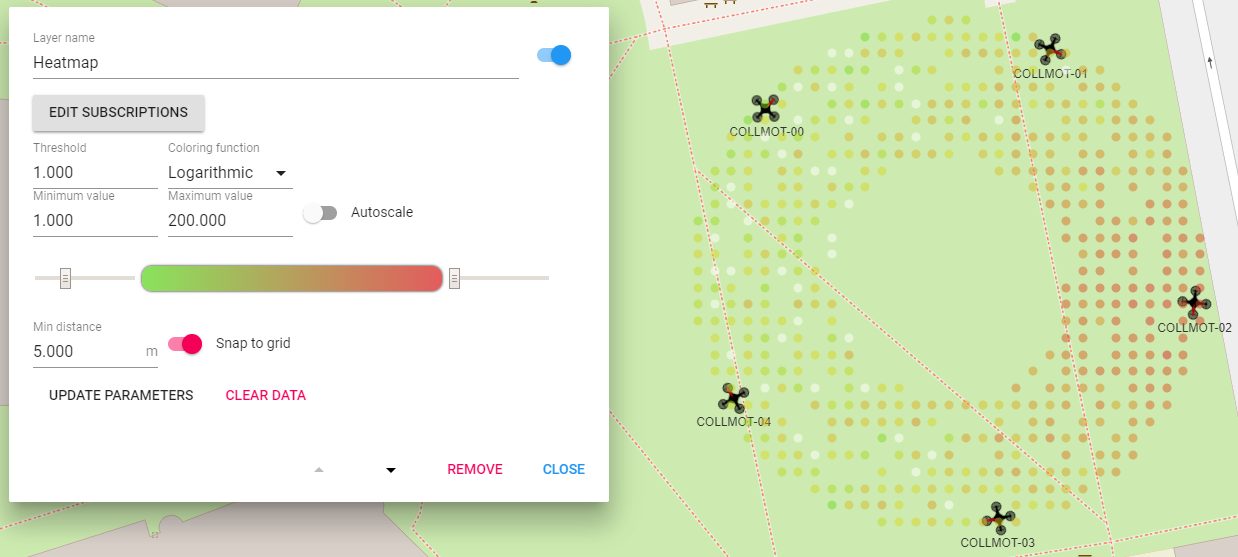
\includegraphics[width=\textwidth]{screenshots/heatmap.png}
  \caption{Egy hőtérkép kinézete}
  \label{fig:heatmap}
\end{figure}


\subsection{Térkép állapotainak elmentése és betöltése}

Az alkalmazás lehetőséget biztosít adott térkép állások (középpont, nagyítás és
elforgatás) tárolására későbbi betöltés céljából. Ehhez felületi elemként
elérhető a kép (\ref{fig:saved_locations}. ábra) bal oldalán látható listát
tartalmazó panel, mely az eddig elmentett opciókat tartalmazza. Egy elemre
rákattintva betölthető az adott állapot, ekkor a térkép animálva átvált egy,
az eltárolt középponttal, nagyítással és elforgatással rendelkező nézetre. A
listaelemek mellett szereplő fogaskerék ikon pedig a kép jobb oldalán látható
dialógusablakban nyitja meg szerkesztésre a kiválasztott helyet. Itt törölhető
is az adott bejegyzés, ha már nincs rá szükség.

Új hely az első elemre ("Add new location") kattintva adható hozzá a
listához. Ekkor a dialógusablak a térkép aktuális állapotának értékeivel
kitöltve nyílik meg, így az könnyen elmenthető, vagy pedig kézzel bevihetőek
kívánt adatok.

\begin{figure}[H]
  \center
  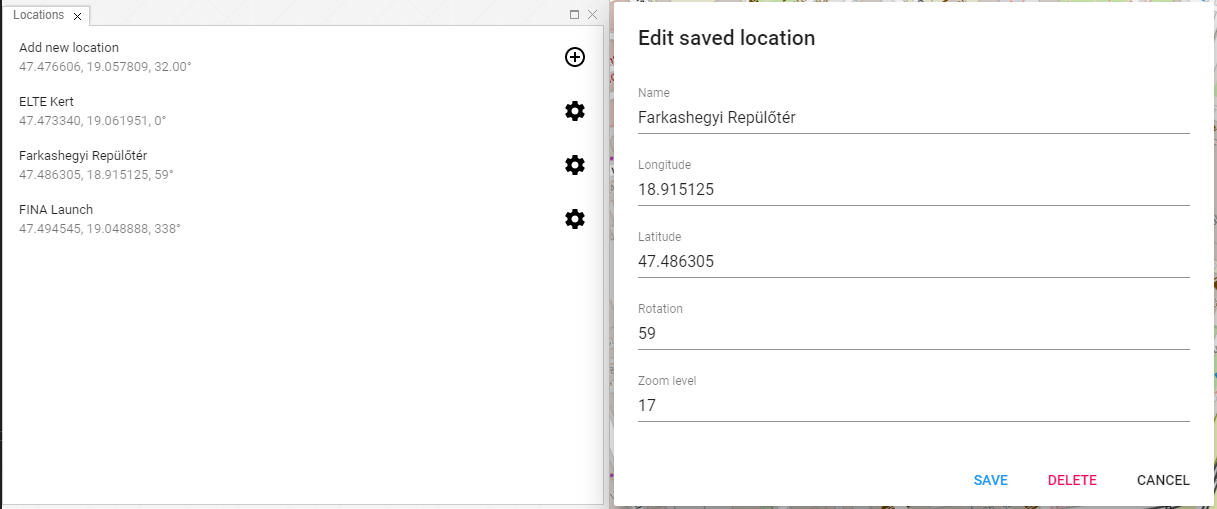
\includegraphics[width=\textwidth]{screenshots/saved_locations.png}
  \caption{A mentett pozíciók panelje és a szerkesztésükre alkalmas dialógusablak}
  \label{fig:saved_locations}
\end{figure}


\subsection{GeoJSON megjelenítése}

A GeoJSON egy elterjedt térképészeti formátum, mely geográfiai objektumok
leírására alkalmas. Drónok vezérlésénél és monitorozásánál szükség lehet előre
megadott létező vagy virtuális terepobjketumok megjelenítésére a térképen, mint
például környező akadályok, épületek, vagy esetleg egy kijelölt repülési zóna.

Ezek megjelenítéséhez egy speciális réteg hozzáadása szükséges. Ez a rétegek
panelen az "Add new layer" gomb megnyomásával lehetséges. Amennyiben az ezt
követően felugró dialógusablakban a GeoJSON opció kerül kiválasztásra, akkor az
alkalmazás felkínálja a réteg beállításait. Megadhatóak a megjeleníteni kívánt
GeoJSON objektum kirajzolásához felhasználandó színek külön a körvonalhoz,
valamint a kitöltéshez, továbbá testreszabható a körvonal vastagsága. A GeoJSON
forrásszöveg elhelyezése is a dialógusablakban lévő szövegdobozban történik,
majd pedig az "IMPORT GEOJSON" gombot megnyomva a forrás által meghatározott
objektum megjelenik a térképen.

GeoJSON formátumú adatok előállításához több különböző szoftver is elérhető, de
akár saját kézzel is elkészíthető az objektumokat leíró forráskód. Az alábbi
illusztráción ( \ref{fig:geojson}. ábra) elhelyezett poligon például a
http://geojson.io címen elérhető szerkesztő segítségével készült.

\begin{figure}[H]
  \center
  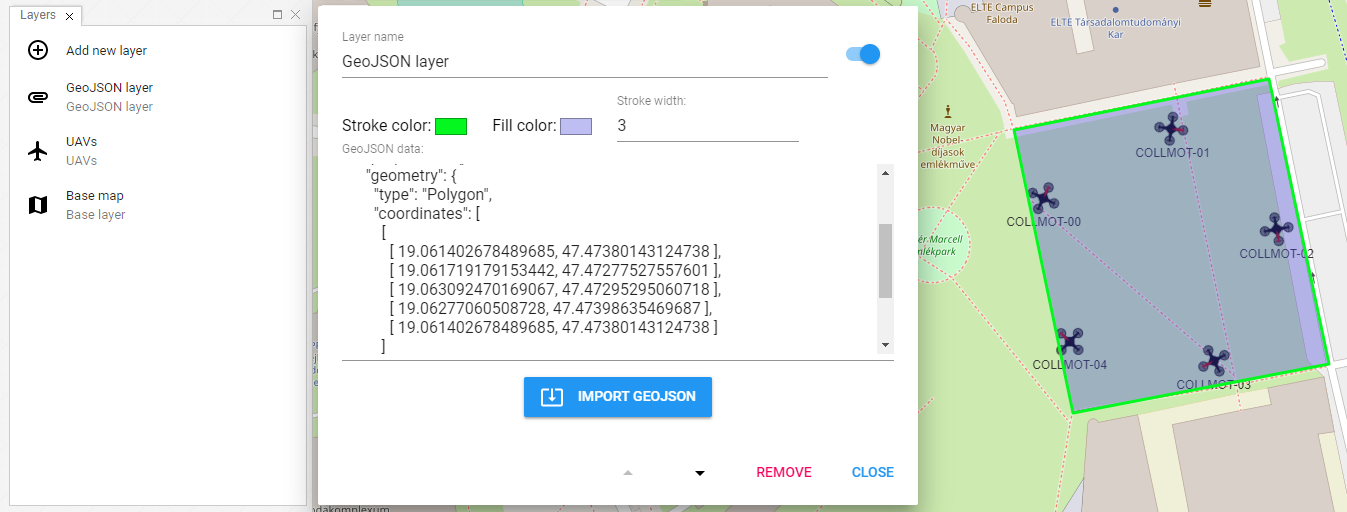
\includegraphics[width=\textwidth]{screenshots/geojson.png}
  \caption{Egy poligont megjelenítő GeoJSON réteg}
  \label{fig:geojson}
\end{figure}

\subsection{Parancsok kiadása drónoknak}

A drónoknak jelenleg négy féle parancs adható ki: felszállás, leszállás,
visszatérés a kiindulópontra valamint kikapcsolás. Ezek a lehetőségek elérhetők
a térképen történő jobb egérgombbal végzett kattintáskor felugró menüből
( \ref{fig:commands}. ábra /\circled{1}), valamint a drónok listáját tartalmazó
panel tetején található eszköztárról ( \ref{fig:commands}. ábra /\circled{2}).
Egy parancs kiadását követően a szerver visszajelzést küld annak végrehajtásának
sikerességéről, ez a válasz pedig bekerül bejegyzésként az eseménynaplóba.

\begin{figure}[H]
  \center
  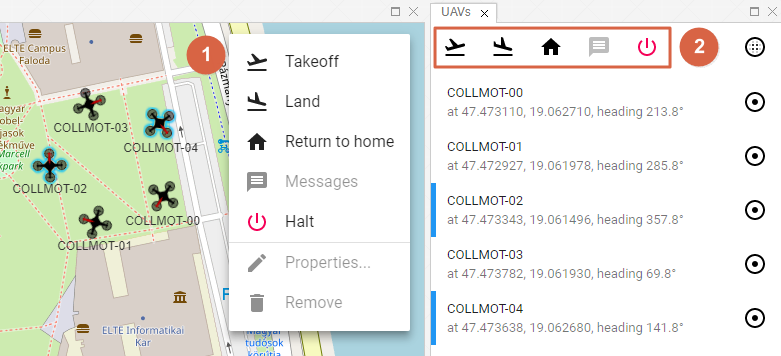
\includegraphics[width=\textwidth]{screenshots/commands.png}
  \caption{A drónoknak történő parancskiadás módjai}
  \label{fig:commands}
\end{figure}


\subsection{Állapotüzenetek kijelzésére alkalmas panel}

A rendszer naplóbejegyzéseit megjelenítő panel alapbeállításként nincs
bekapcsolva, a bal oldali sávról érhető el. A felületre helyezve egy szűrhető
és rendezhető táblázat formájában jeleníti meg az állapotüzenetek listáját.
Alapértelmezetten az üzenetek érkezésének időpontja szerint van csökkenő
sorrendbe rendezve, azonban ez átállítható például az üzenetek szintjei szerinti
rendezésre, továbbá szűrések alkalmazhatók bármelyik oszlopon.

\textit{
  Bővebben a szűrhető és rendezhető táblákról lásd:
  \ref{filterable_sortable_table}
}

\begin{figure}[H]
  \center
  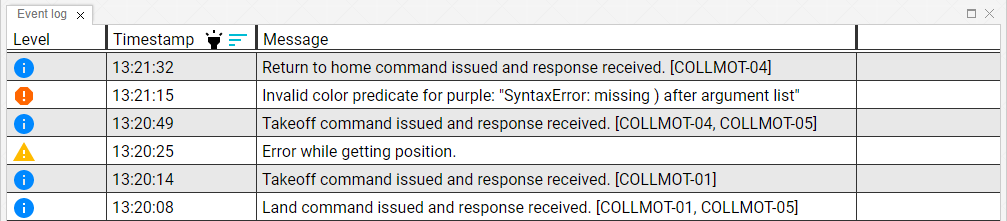
\includegraphics[width=\textwidth]{screenshots/log.png}
  \caption{Példa az állapotüzeneteket tartalmazó lista megjelenésére}
  \label{fig:log}
\end{figure}


\subsection{Drónok színkódolása predikátumok alapján}

A drónok színkodolására vonatkozó predikátumok megadására a kopter piktogramok
megjelenítéséért felelős réteg (UAVs) beállításai között van lehetőség.
Hat szín áll rendelkezésre, ezekhez egy egy JavaScript függvénytörzs rendelhető
hozzá. Az "Apply changes" gomb megnyomásakor a rendszer megvizsgálja a mezők
értékét, és amelyikben hibát talál, azt megjelöli, valamint bejegyézst készít az
eseménynaplóba a hiba pontos szövegéről, a többit pedig elmenti és alkalmazza a
drónokra oly módon, hogy a drónok azonosítóit egyesével paraméterül adja
függvényeknek, és olyan színűre színezi az adott piktogramot, amelyik színhez
tartozó függvény igazra értékelődött ki.

Az alábbi példában (\ref{fig:uav_coloring}. ábra) a lila színhez tartozó
predikátum hibás, a kettőnél kisebb számra végződő azonosítóval rendelkező
koptereket zöldre, a négynél nagyobbakat narancssárgára, a "COLLMOT-02"-es és
"COLLMOT-04"-es drónt pedig kékre színeztük.

\begin{figure}[H]
  \center
  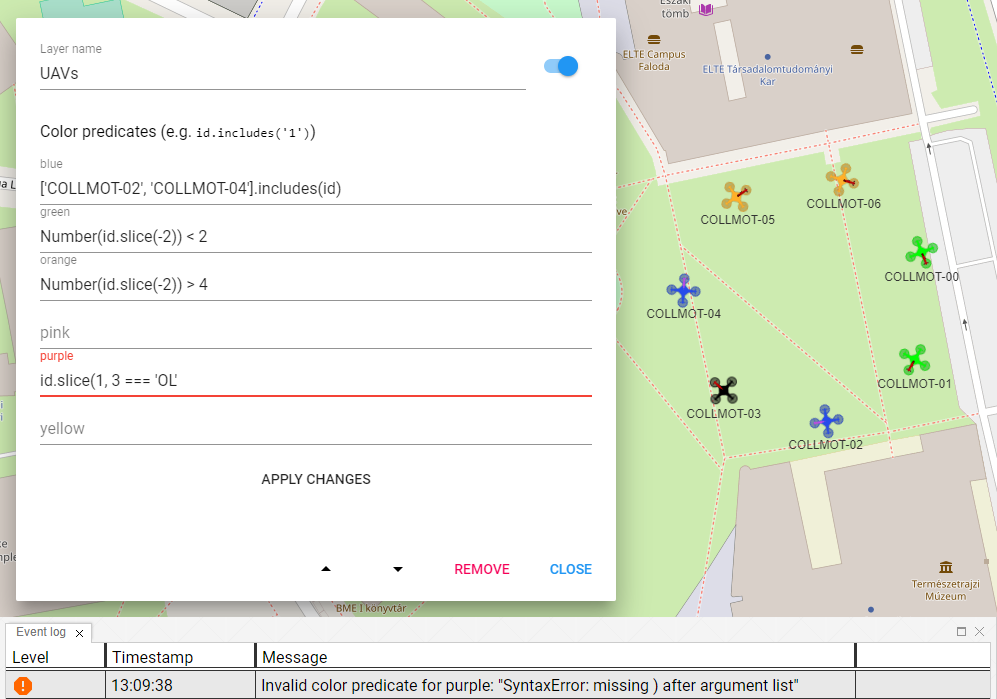
\includegraphics[width=\textwidth]{screenshots/uav_coloring.png}
  \caption{Példa néhány predikátumra}
  \label{fig:uav_coloring}
\end{figure}

\subsection{Drónok részletes aktuális állapotát mutató panel}

A régi karakteres felület előnyének fenntartására, az elérhető információ tömör
formában történő megtekintésére szolgáló "Ground Control View" nézet
alapbeállításként rejtve van, a bal oldali sávról aktiválható. Ekkor egy
szűrhető és rendezhető táblázatként válnak benne elérhetővé a drónok aktuális
adatai.
A név oszlop szöveg típusú szűréssel és rendezéssel rendelkezik, az összes többi
intervallum típusú, így könnyen megkereshetőek például egy adott kritikus
akkufeszültség alatt lévő drónok, vagy mondjuk lehet rendezni őket az
elhelyezkedésük alapján a szélességi és hosszúsági koordinátáik szerint.

\textit{
  Bővebben a szűrhető és rendezhető táblákról lásd:
  \ref{filterable_sortable_table}
}

\begin{figure}[H]
  \center
  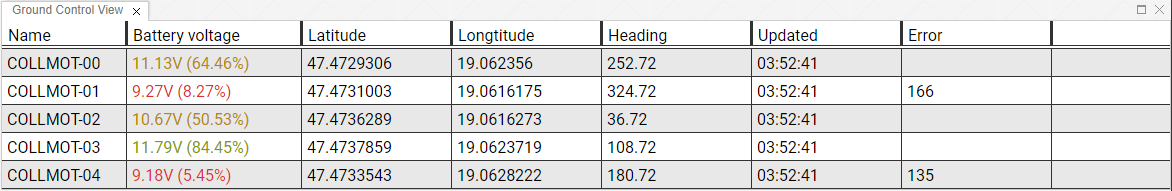
\includegraphics[width=\textwidth]{screenshots/ground_control_view.png}
  \caption{A drónok adatai egy szűrhető és rendezhető táblázatban}
  \label{fig:ground_control_view}
\end{figure}

\subsection{Kliens állomás pozíciójának megjelenítése geolokáció alapján}

Amennyiben a kliens alkalmazást futtató eszköz rendelkezik geolokáció
megállapítására alkalmas szolgáltatással, akkor az "Own location" típusú réteg
hozzáadását követően megjelenik a térképen egy kör alakú kék jelölő.
( \ref{fig:ownlocation}. ábra /\circled{1}) Ha az eszköz képes a pozícióján felül
orientáció megállapítására is például mágneses iránytű segítségével, akkor a
jelölő ennek megfelelően követi az elfordulást is.

\begin{figure}[H]
  \center
  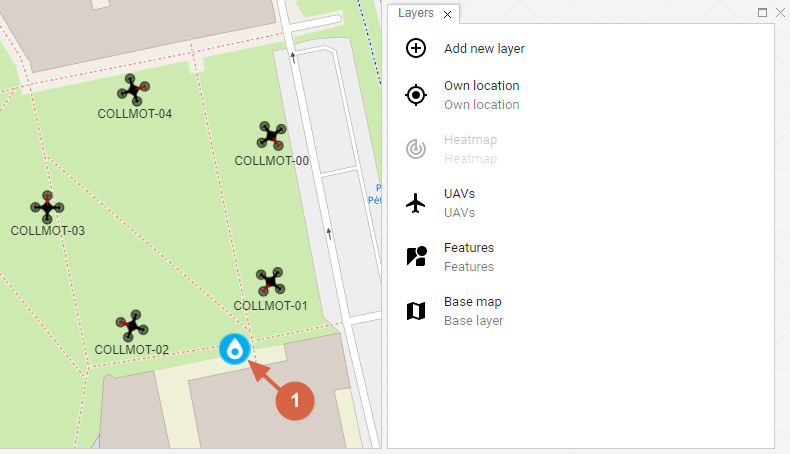
\includegraphics[width=\textwidth]{screenshots/ownlocation.png}
  \caption{A kliens állomás pozícióját mutató jelölő}
  \label{fig:ownlocation}
\end{figure}

\subsection{Billentyűkombinációkkal történő vezérlés}

Az alkalmazásban elérhető Billentyűkombinációk bárhonnan működnek, amennyiben
nincsen aktív beviteli mező. A teljes lista megtekinthető a "?" szimbólum
gépelésére szolgáló Billentyűkombináció lenyomásával.

(Ide írjam le a teljes listát?)


\subsection{A szűrhető és rendezhető táblák kezelése}
\label{filterable_sortable_table}

Szűrhető és rendezhető táblázaton alapul a drónok részletes állapotát mutató
panel, valamint a naplóbejegyzések megjenítésére szolgáló lista.

Az ilyen fajta táblázatok oszlopainak fejléce fölé víve az egeret kettő gomb
válik láthatóvá. Az első az adott oszlop szerinti szűrésre, a második pedig az
adott oszlop szerinti rendezésre szolgál. A rendezés aktiválása után annak
iránya megfordítható ikonra történő ismételt kattintással.

Szűrés szempontjából három különböző fajtájú oszlop létezik.
Ezek működése illusztrálva az eseménynapló panel segítségével.
(Eredeti állapothoz lásd: \ref{fig:log}. ábra).

\begin{itemize}
  \item Előre megadott lehetőségek halmazából felvett értékek
  \begin{figure}[H]
    \center
    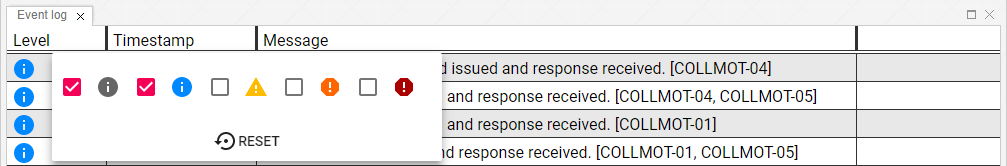
\includegraphics[width=\textwidth]{screenshots/filtered_table_list.png}
    \caption{Csak az információ típusú naplóbejegyzések megjelenítése}
    \label{fig:filtered_table_list}
  \end{figure}

  \item Intervallum típusú értékek
  \begin{figure}[H]
    \center
    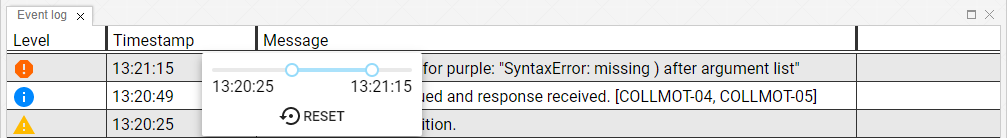
\includegraphics[width=\textwidth]{screenshots/filtered_table_range.png}
    \caption{Csak a 13:20:25 és 13:21:15 közötti naplóbejegyzések megjelenítése}
    \label{fig:filtered_table_range}
  \end{figure}

  \item Szöveg típusú értékek
  \begin{figure}[H]
    \center
    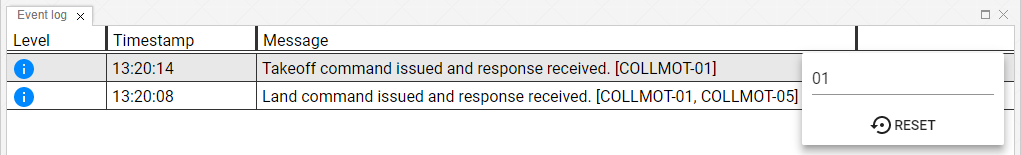
\includegraphics[width=\textwidth]{screenshots/filtered_table_text.png}
    \caption{Csak a 01-es drónnal kapcsolatos naplóbejegyzések megjelenítése}
    \label{fig:filtered_table_text}
  \end{figure}
\end{itemize}


